\section{Combined Attack}
After the suggested protocol update the honest prover cannot contain any thorny blokcs in his suffix NIPoPoW even if these blocks are part of his chain $\chain_B$. The adversary may exploit this fact as follows. She tries to suppress honestly generated blocks in $\chain_B$, in order to reduce the blocks that can represent the honest chain in a proof. In parallel, while she mines suppressive thorny blocks on $\chain_B$ she can still use her blocks in her NIPoPoW proofs, by chainsewing them. Consequently, even if a suppression attempt does not succeed, in case for example that a second honestly generated block is soon enough published, she does not lose the mining power spent but can still utilize it by including the block in her proof.

More in detail, consider that the adversary wishes to attack a specific block level $\mu_B$ and generate a NIPoPow proof containing a block $b$ of a fork chain which contains a double spending transaction. Then she acts as follows. She may mine on her fork chain $\chain_\mathcal{A}$ but when she observes a $\mu_B$-level block in $\chain_B$ she tries to mine a thorny block on $\chain_B$ in order to suppress this $\mu_B$ block. This thorny block contains an interlink pointer which jumps onto her fork chain. If the suppression succeeds she has managed to damage the $\mu_B$ superchain and, at the same time, to mine a block that she can afterwards use in her proof. If the suppression does not succeed she can still use the thorny block in her proof. The above are illustrated in Figure \ref{fig:attack_after_update}.

\begin{figure}[h!]
	\begin{center}
    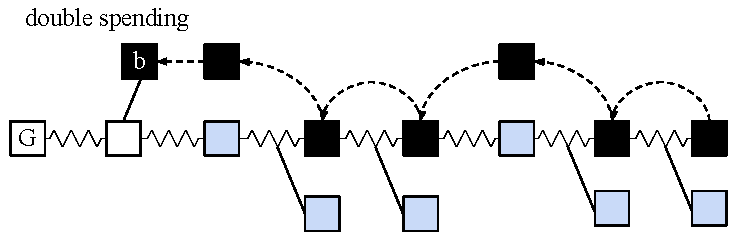
\includegraphics[width=0.95\columnwidth]{figures/attack_after_update-crop.pdf}
	\end{center}
	\caption{The adversary suppresses honestly generated blocks and chainsews thorny blocks in $\chain_B$. Blue blocks are honestly generated blocks of some level of attack. The adversary tries to suppress them. If the suppression is not successful, the adversary can still use the block she mined in her proof.}
	\label{fig:attack_after_update}
\end{figure}

The described attack consists a combined attack since both suppression and chainsewing are utilized. This combined attack forces us to consider the Velvet Honest Majority Assumption of (1/4)-bounded adversary, so as to guarantee that the unsuppressed blocks in $\chain_B$ suffice for constructing winning NIPoPoW proofs against the adversarial ones.